
\section{Discriminative vs. Generative Models}\label{discriminative_modelinmg}
\subsection{Overview}
Machine learning models can be classified into two main categories, discriminative and generative models. Simply put, a discriminative model makes predictions based on conditional probability $p\left(y|\bx\right)$ and is either used for classification or regression problems. In other words discriminative models distinguishes the decision boundary between the
classes.  It corresponds to learning parameters maximizing conditional probability
distribution $p(y|\bx)$. In opposition, a generative model revolves around the distribution of a dataset to return a probability for a given example. Rather than
looking at classes and trying to find something to separate them, it focuses
only on the one class at the time and builds a model what that certain class looks like, than turns attention to the other class. To express it more formally, generative models learns parameters maximizing $p\left(\bx|y \right)$ and $p\left(y\right)$. Since
\begin{align}\label{eq:prob_decompostion}
p\left(\bx,y\right) = p\left(\bx|y\right)\cdot p\left(y\right),
\end{align}
with joint PDF it is possible to generate new $\left(\bx',y'\right)$ pairs. In some cases, using the second decomposition $p\left(\bx,y\right) = p\left(y|\bx\right)\cdot p\left(\bx\right)$ is also an option.  Note that in an unsupervised setting the task is reduced to inferring only $p\left(\bx\right)$.
\begin{figure}[h]
	\centering
	\begin{minipage}{.5\textwidth}
		\centering
		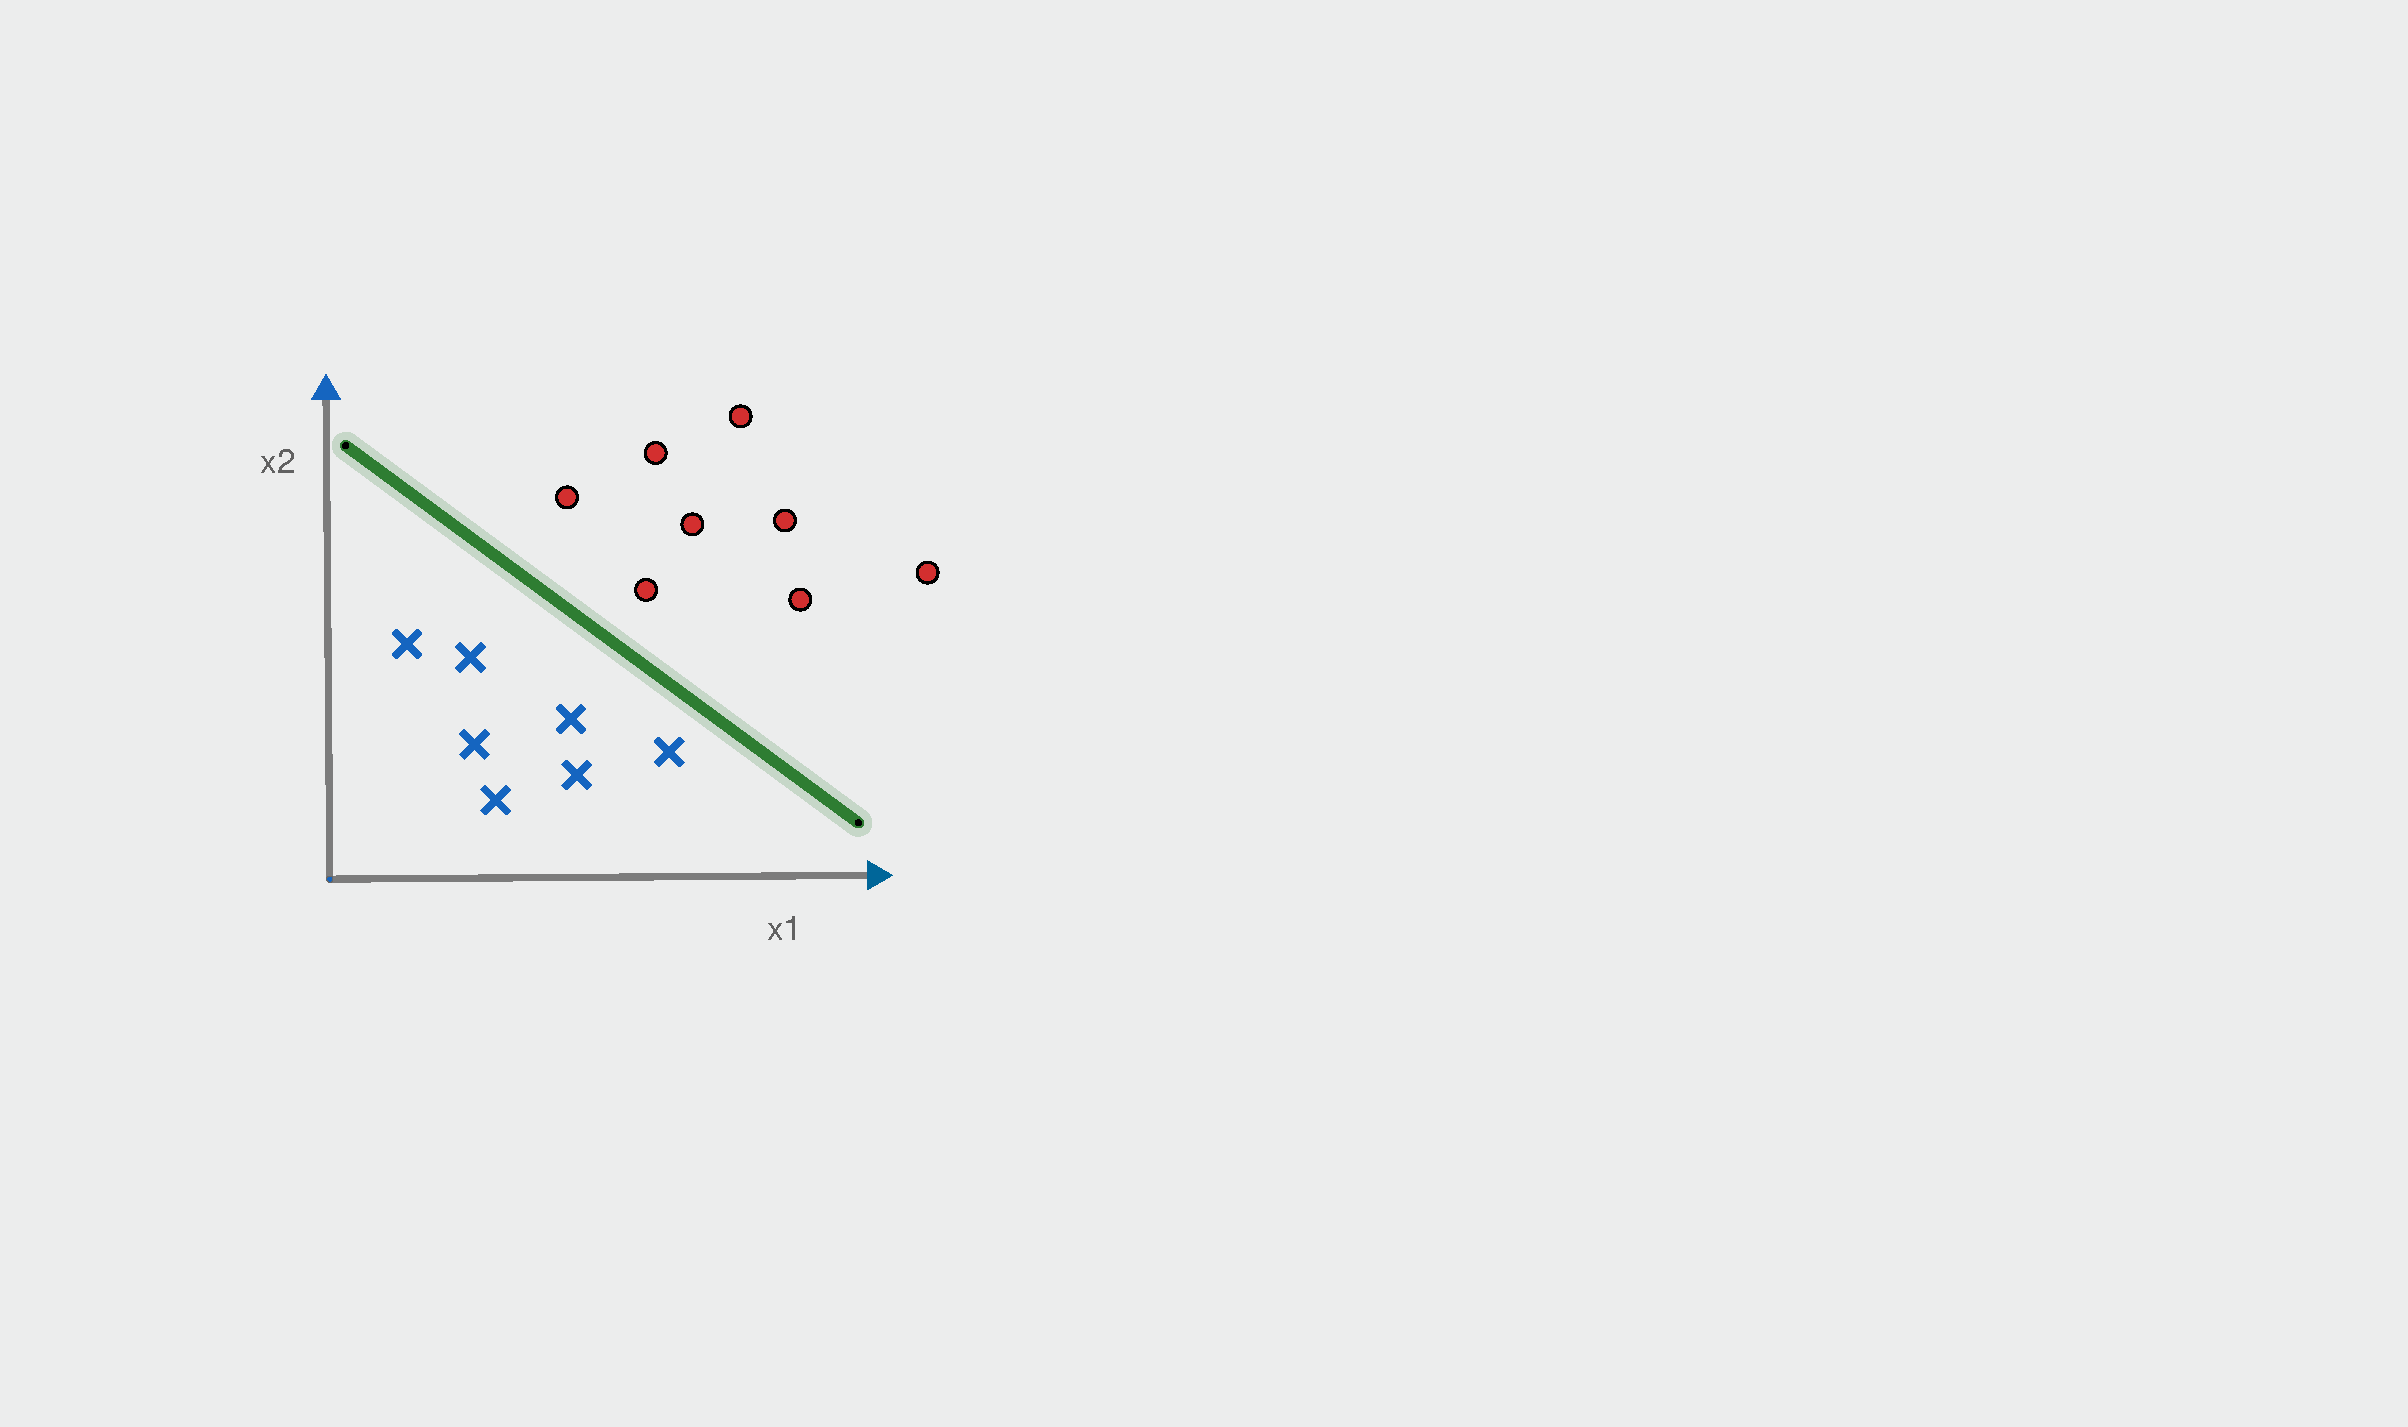
\includegraphics[trim = 4cm 8cm 24cm 6cm, clip = true, totalheight=0.26\textheight]{plots/Images/discriminative_model.pdf}
		\captionof{figure}{Discriminative approach. }
		\label{fig:test1}
	\end{minipage}%
	\begin{minipage}{.5\textwidth}
		\centering
		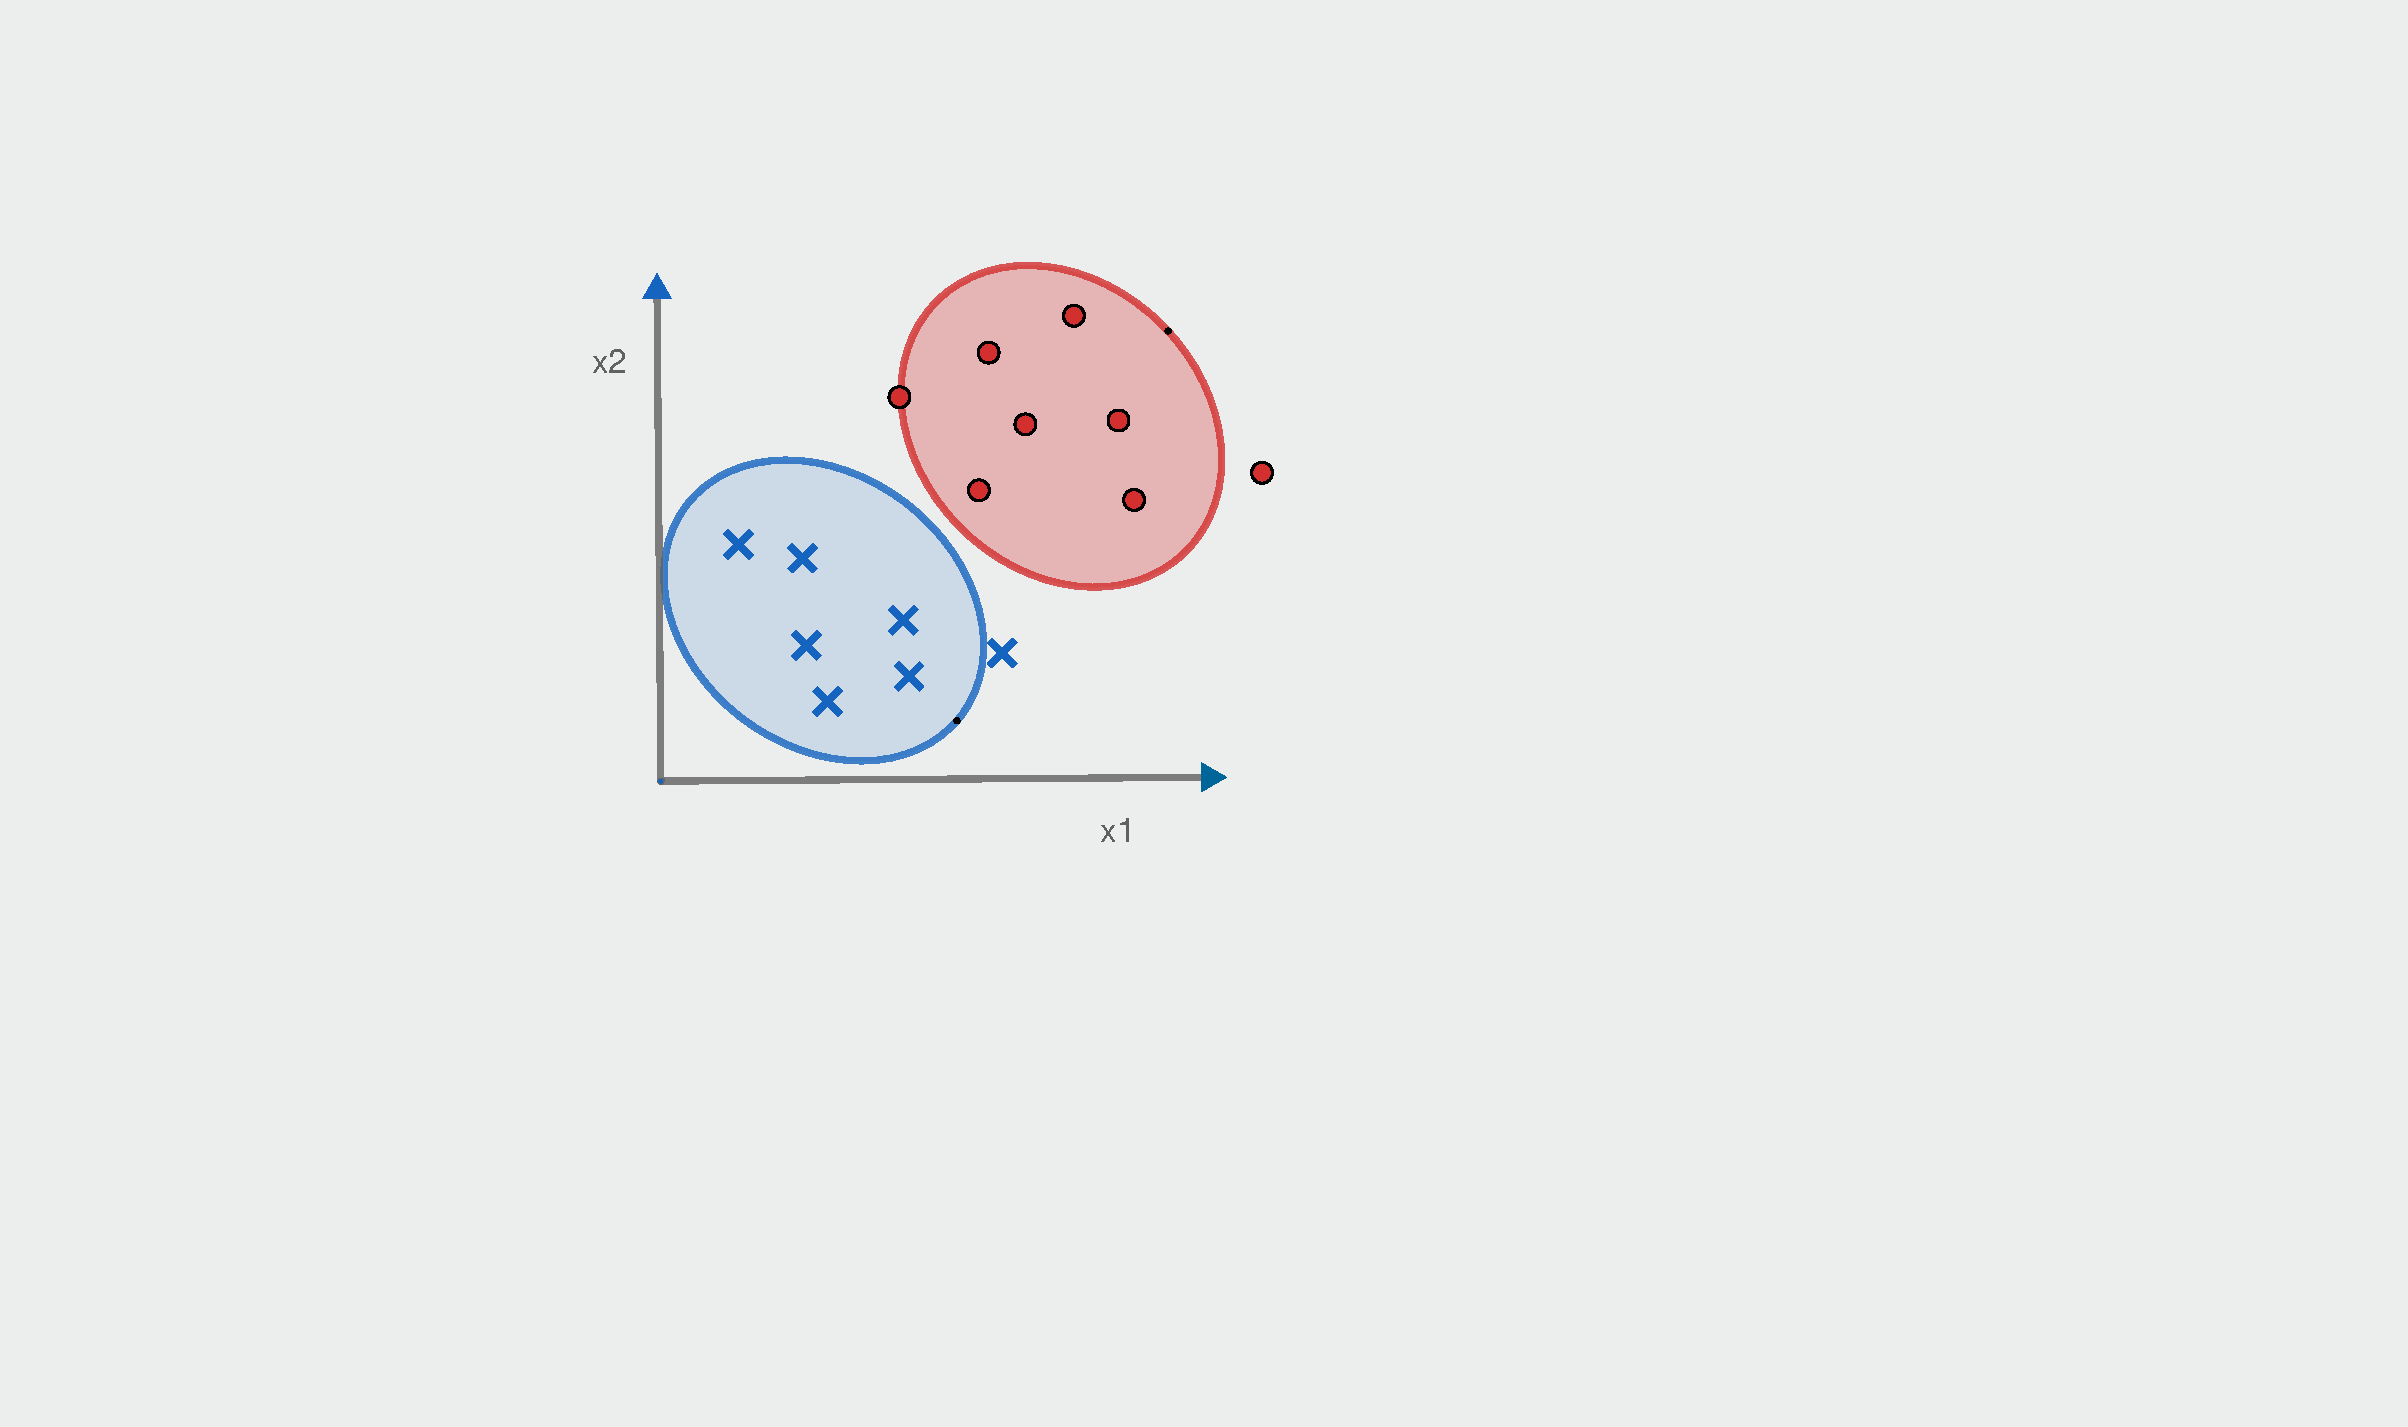
\includegraphics[trim =9.6cm 9.6cm 19cm 4cm, clip = true, totalheight=0.26\textheight]{plots/Images/generative_model.pdf}
		\captionof{figure}{Generative approach.}
		\label{fig:test2}
	\end{minipage}
%\caption{Discriminative and Generative approach.}
\end{figure}
\subsection{Discriminative modeling}
In this section, we review basics of discriminative modeling that was proposed in \cite{HDGEmain}. Given a data distribution via probability density $p(\boldsymbol{x})$ and a label distribution with probability density $p(y|\boldsymbol{x})$ containing $C$ categories. In other words, variable $y$ is now cathegorical taking on $C$ possible values and comes from a finite set $\mathcal{C}$.  A classification problem is typically solved using a parametric function $f_{\boldsymbol{\theta}} : \mathbb{R}^D \to \mathcal{C}$, where $\boldsymbol{\theta}$ denotes parameters of the model. In practice, function $f_{\boldsymbol{\theta}}$ is often used in the form of $\mathbb{R}^D \to  \mathbb{R}^C$. This function maps each data point $\boldsymbol{x} \in \mathbb{R}^D$ to $C$ real-valued numbers known as logits. One has to keep in mind that $\mathbb{R}^C$ is allowed here due to the utilization of \emph{one-hot encoding}, which will be explained in section \ref{OHE}. Logits are used to parametrize a categorical distribution via the function
\begin{equation}\label{softmax}
	q_{\boldsymbol{\theta}}\left(y|\boldsymbol{x}\right) = \frac{\exp\left({f_{\boldsymbol{\theta}}\left(\boldsymbol{x}\right)[y]}\right)}{\sum_{i=1}^C\exp\left({f_{\boldsymbol{\theta}}\left(\boldsymbol{x}\right)[y_i]}\right)},
\end{equation}
which is known as the Softmax function. Note that the convention $f_{\boldsymbol{\theta}}\left(\boldsymbol{x}\right)[y]$ means the $y^{\mathrm{th}}$ element of the $f_{\boldsymbol{\theta}}\left(\boldsymbol{x}\right)$. For learning $f_{\boldsymbol{\theta}}$ is usually minimized cross-entropy loss 
\begin{equation}\label{crossentropy}
	\min_{\boldsymbol{\theta}}- \mathbb{E}_{ p_{\mathrm{data}}(\boldsymbol{x},y)}\left[\log q_{\boldsymbol{\theta}}\left(y|\boldsymbol{x}\right)\right].
\end{equation} 
Rationale for this objective comes from minimizing the Kullback-Leibler divergence with a target distribution $p(y| \boldsymbol{x})$ \cite{KL}. In general,
Kullback-Leibler divergence, for distribution functions $\Psi$ and $\Pi$ with corresponding PDFs $\psi$ and $\pi$, is defined as
\begin{equation}
D_{\mathrm{KL}} \left(\Psi || \Pi \right) = \int \psi(x)\log\frac{\psi(x)}{\pi(x)}\d{x} = \mathbb{E}_{x\sim \psi} \left[\log\frac{\psi(x)}{\pi(x)} \right],
\end{equation}
which can be further rewritten in the form
\begin{equation}
	 \mathbb{E}_{x\sim \psi} \left[\log\frac{\psi(x)}{\pi_{\boldsymbol{\theta}}(x)} \right] = \mathbb{E}_{x\sim \psi} \left[\log \psi(x) \right] - \mathbb{E}_{x\sim \psi} \left[\log \pi_{\boldsymbol{\theta}}(x) \right],
	\end{equation}
where subscript $\boldsymbol{\theta}$ emphasizes that $\pi_{\boldsymbol{\theta}}(x)$ is our approximative density we get to control. Note that
the first term does not depend on $\bt$ and therefore minimizing either CE or KL divergence is equivalent. Finally, by minimizing with respect to $\pi_{\boldsymbol{\theta}}(x)$ we obtain
\begin{equation}
\min_{\boldsymbol{\theta}} D_{\mathrm{KL}} \left(\Psi || \Pi \right) = \min_{\boldsymbol{\theta}} - \E_{x\sim \psi}\left[\log \pi_{\boldsymbol{\theta}}\left(x\right)\right].
\end{equation}
For clarity, the expected value will be discussed. In practise, it is dealt with discrete data, so the term  $\E_{x\sim \psi}\left[\log \pi_{\boldsymbol{\theta}}\left(x\right)\right]$ takes the form
\begin{equation}
    \E_{x\sim \psi}\left[\log \pi_{\boldsymbol{\theta}}\left(x\right)\right] = \sum_{i=1}^N \psi(x_i)\log\pi_{\bt}\left(x_i\right).
\end{equation}
\subsection{One-hot encoding}\label{OHE}
 Machine learning (ML) algorithms can misinterpret the numeric values of labels if there exists any hierarchy between them. One-hot encoding is a very common approach how to deal with this issue, in order to improve the algorithm performance. \\
 Each unique category value is transformed into a new column and these dummy variables are then filled up with 0 or 1 (0 for FALSE and 1 for TRUE). Transformation of a label encoding to the one-hot encoding is illustrated in following tables \ref{tab:LE} and \ref{tab:OHE}. \\
 However, this method has its own downsides. For example, it creates new variables and if there exists many unique category values, models have to deal with large amount of predictors, causing so-called \emph{Big-p problem} \cite{Bigp}. Also, one--hot encoding causes multi-colinearity between the individual variables, which may lead to reducing model's accuracy. 
 \begin{table}[h]
 	\centering
 	\begin{tabular}{|l|l|l|}
 		\hline
 		Food Name & Categorical \# & Calories \\ \hline
 		Pizza     & 1              & 266      \\ \hline
 		Hamburger & 2              & 295      \\ \hline
 		Caviar    & 3              & 264      \\ \hline
 	\end{tabular}
 	\caption{Example of label encoding.}
 	\label{tab:LE}
 \end{table}

\begin{table}[h]
	\centering
	\begin{tabular}{|l|l|l|l|}
		\hline
		Pizza & Hamburger & Caviar & Calories \\ \hline
		1     & 0         & 0      & 266      \\ \hline
		0     & 1         & 0      & 295      \\ \hline
		0     & 0         & 1      & 264      \\ \hline
	\end{tabular}
	\caption{Example of one--hot encoding.}
	\label{tab:OHE}
\end{table}
\subsection{Generative modelling}
